\chapter{Evaluation}
\label{chap:evaluation}

This chapter will try to evaluate the new threats disclosed by the prototype.
First, some sample attacks are driven, then they are analyzed. Last, this
chapter will try to extrapolate the possibility of further social engineering
attacks.

\section{Demonstration of attacks using the prototype}

This section wants to demonstrate how the prototype, which was
developed in the previous chapter, can assist a social engineering attack.
Therefore, the attacks previous described in chapter \ref{chap:attacks} are
repeated together with the aid of the prototype.

\section{Phishing mail}

The attack itself was already described in section \ref{sec:phishing_mail}. It
will now be driven against a sample profile on \Twitter{} using the prototype.
The attack is visually represented in figure \ref{fig:evaluation_phishing}.
The following data is therefore needed:

\begin{itemize}
  \item Real name of the victim
  \item E-mail address of the victim
  \item The Knowledge, that the victim is a customer of an electronic
  payment service, like \textit{PayPal}, \textit{Amazon} or \textit{eBay}
\end{itemize}

The attacker now simply starts off with a simple keyword search, as he is not
interested in a specific person (at least for now). Therefore he runs:

\lstset{language=bash}
\begin{lstlisting}
$ python prototype.py -k "paypal"
\end{lstlisting}

This opens a new website on \url{http://search.twitter.com}, which shows the
attacker people, who quoted the word \textit{paypal} in one of their messages.
The attacker now picks a person with the username \textit{petersample}, who writes

\begin{quote}
did really some transactions over paypal this week, works really great!
\end{quote}

As the attacker now has a individual he can attack, he is interested in more
information. Therefore he runs:

\lstset{language=bash}
\begin{lstlisting}
$ python prototype.py -u "petersample"
\end{lstlisting}

\begin{figure}[htb]
  \begin{center}
    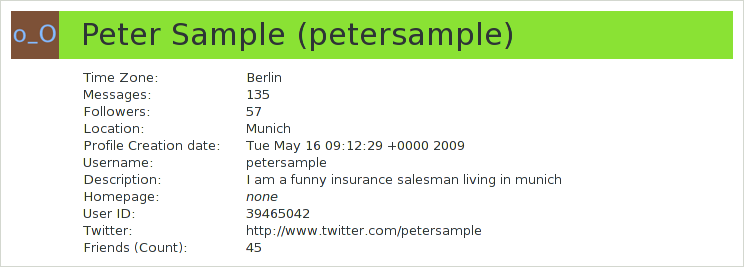
\includegraphics[width=\textwidth]{prototype_user}
    \caption{Prototype output: general information about a user.}
    \label{fig:prototype_user}
  \end{center}
\end{figure}

This now produces a fact sheet about Peter Sample. As the attacker already
knows, that the victim is using \textit{PayPal}, he just needs the real name
and the e-mail address. The output of the prototype is displayed in figure
\ref{fig:prototype_user}. The attacker now knows the real name. The e-mail
address was also found by the prototype and is displayed in figure
\ref{fig:prototype_mail}. Now, every data needed for the phishing mail is
acquired and the attacker can begin to send the e-mails out. Just like described,
it is also possible to include Peter Sample's friends, if they are using
\textit{PayPal} too. This is simply done by redoing the attack on Peter
Sample's friends, which the prototype also outputs.

\begin{figure}[htb]
  \begin{center}
    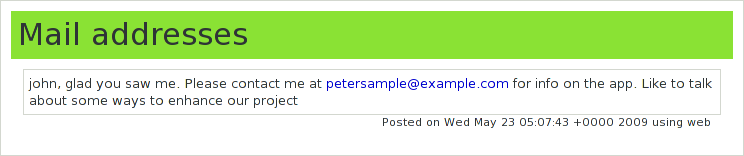
\includegraphics[width=\textwidth]{prototype_mail}
    \caption{Prototype output: e-mail address was found.}
    \label{fig:prototype_mail}
  \end{center}
\end{figure}

\begin{figure}[ht]
  \begin{center}
    \includegraphics[width=0.75\textwidth]{evaluation_phishing.1}
    \label{fig:evaluation_phishing}
    \caption{Activity diagram of the phishing attack.}
  \end{center}
\end{figure}

\section{Insider attack}

In the attack described in section \ref{sec:insider_attack},
the attacker starts again with a keyword search, as he wants to find an
employee of Sample Company Inc. Quite quickly he finds petersample, who seems to work
for that company. He launches to information retrieval about that user and gets
an output like in figure \ref{fig:prototype_user2}.

\begin{figure}[htb]
  \begin{center}
    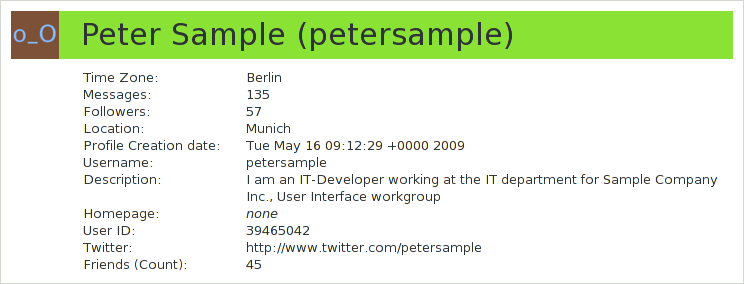
\includegraphics[width=\textwidth]{prototype_user2}
    \caption{Prototype output: general information about an employee of Sample
    Company Inc.}
    \label{fig:prototype_user2}
  \end{center}
\end{figure}

He now knows the real name, the
company and department Peter Sample works for, the workgroup inside the
company, and has an approximate idea where the victim could live. A text search
about some phone specific terms, produces an output like showed in figure
\ref{fig:prototype_phone}. The employee number is trickier to get, as one must
rely that the employee posts this number into a message. In this scenario, this
is not the case and the social engineer has to call Peter Sample at his phone
number.

\begin{figure}[htb]
  \begin{center}
    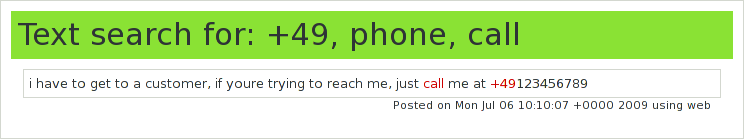
\includegraphics[width=\textwidth]{prototype_phone}
    \caption{Prototype output: text search about phone specific terms.}
    \label{fig:prototype_phone}
  \end{center}
\end{figure}


\begin{figure}[htb]
  \begin{center}
    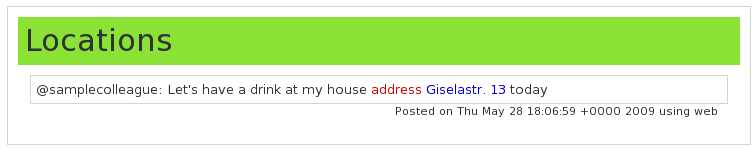
\includegraphics[width=\textwidth]{prototype_residence}
    \caption{Prototype output: the residence is revealed.}
    \label{fig:prototype_residence}
  \end{center}
\end{figure}
The prototype also shows the times, showed in figure
\ref{fig:prototype_times}, Peter Sample mostly writes his
updates and therefore is most probably available, and not having holidays for
example. This was also done in the original scenario, however this time much
less information is needed, as most data can already be get out of the social
network. Next, he needs the residence of Peter Sample, which the prototype also
supports and is displayed in figure \ref{fig:prototype_residence}.

\begin{figure}[htb]
  \begin{center}
    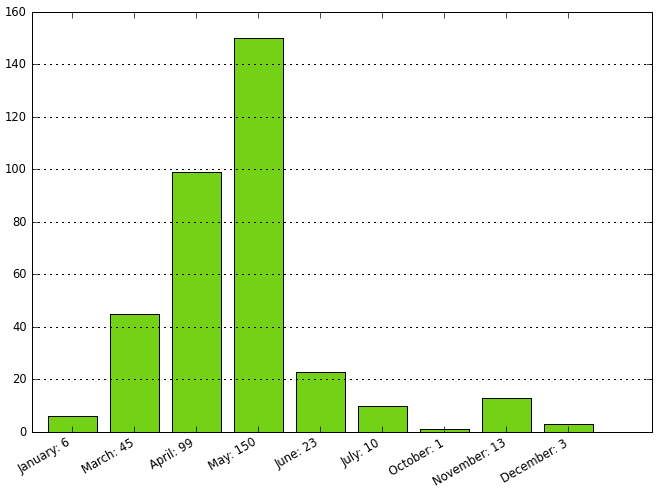
\includegraphics[width=0.49\textwidth]{prototype_times_month} 
    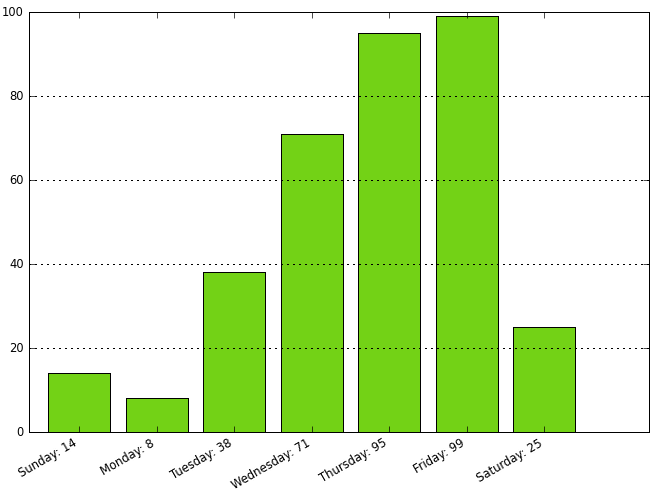
\includegraphics[width=0.49\textwidth]{prototype_times_day} 
    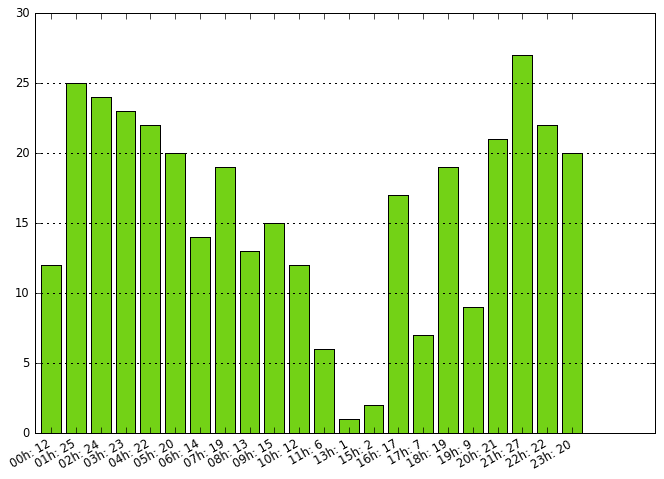
\includegraphics[width=0.49\textwidth]{prototype_times_hour}
    \caption{Prototype output: the average times a user writes his updates: months,
    week, day average.}
    \label{fig:prototype_times}
  \end{center}
\end{figure}

The use of security devices and server names is either determined by the phone
call mentioned above or by a text search. A text search works quite good, as
many people write some message about not working things, like a broken
connection to their development server or that they dislike special security
devices. This data can be harvested like the phone number before.

The company structure, like the managers name and colleagues of the employee
can be determined by analyzing the hidden friends network and the replies the
employee made. By further analyzing the friends networks, replies and applying
the same data retrieval as above, a quite detailed company and employee
structure can be determined.

As in the original scenario, the attacker now just has to wait for a snow storm
in the area of the residence of the employee, which is easy to check, as he
has the residence address.

\section{The bank heist}

The scenario described in section \ref{sec:bank_heist} is quite different from
the others, as it requires data, which normally is or at least should not
published. While the first part of the scenario, like names, phone numbers and
departments is possible to extract either by using the prototype or by directly
doing social engineering attacks, the daily wire transfer code is not
published. While it still might be possible for a social engineer to get the
code, it is not possible to do that over a social network like \Twitter{}, as
this sensitive data is not published. Though, the prototype can still save a
lot of effort, for example by determining the structure of the company or
analyzing company employees.


\section{General feasibility and extrapolation of attacks}

Attacks and information retrieval are possible with the prototype. That was
shown in the above scenarios. One big barrier though remains private and
sensitive data, at least if a user of a social network identifies specific data
as sensitive. However many user do not, and post e-mail addresses, residence
addresses, phone numbers, passwords and further more.

Harvesting this data automatically makes the life of a social engineer
definitely easier, as he just has to execute the attack and is no more
constrained to do a information research beforehand. When it comes to sensitive
data, a prototype like the one introduced, can still help to gain data around
the sensitive data, like company information or user specific information.

With it's plugin architecture, the prototype is easily extendible and more data
and analysis can be simply done. For this prototype the \Twitter{} social
network was chosen, however other famous social networks are possible too.
Putting together more social networks and possibly search engines too, this can
give a more complete picture of a victim.

Most of the effort put into the prototype was to do text mining. Though is
also a lot of optimization possible regarding text analysis. However, the
prototype was able to gain much more information, than a simple or even a more
complex text search engine could do, for example a search engine. The prototype
offers a wide range of analysis possibilities, all suited for special social
engineering attacks. This was shown in the previous sample attacks.

The prototype did get all data legally and can operate almost anonymously, as
he will not be tracked, with the small amount of data it fetches. Though it has
a big effect and can lead to very dangerous and above all easy to accomplish
attacks.

\section{New threats}

Critical attacks based on social engineering techniques are possible, that was
demonstrated. The question however is now, what new threats this work
discovered, along with other researches. As already stated before, the threat
does not come out of the possibility to gather information, it comes out of the
social engineering attacks, which are based on such information. The work
showed, that it is possible to gather large amount of sensitive data of several
users fast and almost anonymously. This means, that the research phase of a
social engineering attack can be almost replaced and done automatically,
depending on the attack scenario. By fetching the data automatically and
without knowledge of the victim, the attacker can prepare the attack while
remaining hidden and not exposing himself to the danger of being discovered.

Taking this approach one step further, automatic harvesting and attacks could
be a future scenario. An attacker could define some social engineering attacks,
like the phishing mail attack, which was showed before, and let them run over a
social network. As there is no way to stop such an attack, this would have an
enormous impact. Brown et al.~\cite{brown2008} for example were able to create
a context-aware phishing mail attack inside a social network, which was
extremely successful. This scenario however is not just restricted to phishing
mail attacks, but is open to all social engineering attacks, where the attacker
no longer chooses a suitable attack for a victim, but the victim chooses the
attack by himself, by just exposing sensitive data.
